%%%%%%%%%%%%%%%%%%%%%%%%%%%%%%%%%%%%%%%%%%%%%%%%%%%%%%%%%%%%%%%%%%%%%%%%%%%%%%%%%%%%%%
\begin{project}
{Focus meter}
{Mobile application for measuring meeting participants focus and engagement.}
{
Mobile application and web server that would allow to
monitor participants mood. Based on the survey meeting
agenda could be changed.
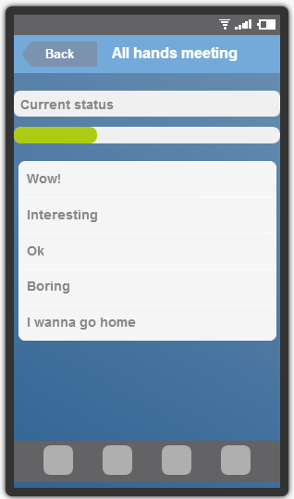
\includegraphics[height=10cm]{focus_meter.png}
}
{Windows Phone/Android}
{Mateusz Jaworski}
{1 semester}
{1-4}
\end{project}
%%%%%%%%%%%%%%%%%%%%%%%%%%%%%%%%%%%%%%%%%%%%%%%%%%%%%%%%%%%%%%%%%%%%%%%%%%%%%%%%%%%%%%
\begin{project}
{Anonymous surveys}
{Web application for making anonymous surveys}
{
Application should allow survey creation for dedicated group of people. 
Neither survey author nor participants could be able match people with answers.
Participants should be able to verify if their answers were not modified. 
Security of the solution should be provable. Questions can have a form of T/F
checkboxes, comboboxes and text fields (in this case we can assume that the
participants are aware of the risk of revealing themselves).
}
{-}
{Mateusz Jaworski}
{1 semester}
{1-4}
\end{project}
%%%%%%%%%%%%%%%%%%%%%%%%%%%%%%%%%%%%%%%%%%%%%%%%%%%%%%%%%%%%%%%%%%%%%%%%%%%%%%%%%%%%%%
\begin{project}
{DocsDB}
{Database system that will be able to store and index any popular form of
documents like mails, microsoft office formats, pdfs.}
{
Web application with simple human interface based on google's search engine and
RESTful API for feeding the database.
Application should provide full-text search for the stored documents which can be based on Elasticsearch database.
Possible extensions:
\begin{itemize}
  \item[-] ability to fetch and index e-mail boxes
  \item[-] ability to index files from disks
\end{itemize}
Useful links
\begin{itemize}
  \item[-] \url{http://www.elasticsearch.org}
  \item[-] \url{http://tika.apache.org}
  \item[-] \url{http://aperture.sourceforge.net}
\end{itemize}
}
{NoSQL database}
{Mateusz Jaworski}
{1 semester}
{1-4}
\end{project}
%%%%%%%%%%%%%%%%%%%%%%%%%%%%%%%%%%%%%%%%%%%%%%%%%%%%%%%%%%%%%%%%%%%%%%%%%%%%%%%%%%%%%%
\begin{project}
{OCR for graphs and structured data}
{Optical character recognition library for conversion of handwritten graphs and structured data into digital format.} 
{ 
Graphs can have some fixed form and limited number of elements to recognise, i.e. 
they can consist of arrows and boxes filled with text. They can be converted to any text format.
 For structured data you can define some abstract structure like: 'text and
 number in circle on the right hand side' and application should try to match
 those with the photo.
}
{-}
{Mateusz Jaworski}
{1 semester}
{1-3}
\end{project}
%%%%%%%%%%%%%%%%%%%%%%%%%%%%%%%%%%%%%%%%%%%%%%%%%%%%%%%%%%%%%%%%%%%%%%%%%%%%%%%%%%%%%%
\begin{project}
{Augmented notification system}
{Composite solution for distributing notifications via light, sound and touch.}
{
The system could have a form of central controller with many different 
peripheral devices that would be used for handling notifications and alarms. 
The main aim is to present status of continuous integration server in a highly visible manner. 
Those peripheral devices could have a form of RGB lamps, signal lights (same as used for the traffic control) or usb rocket launchers.
}
{-}
{Mateusz Jaworski}
{1 semester}
{1-4}
\end{project}
%%%%%%%%%%%%%%%%%%%%%%%%%%%%%%%%%%%%%%%%%%%%%%%%%%%%%%%%%%%%%%%%%%%%%%%%%%%%%%%%%%%%%%
\begin{project}
{Mobile application facilitating meeting data exchange}
{Application for Android or Windows Phone which facilitates sharing photos,
videos and other files between meeting participants.} 
{
Project can be implemented in many various ways. Host of the meeting can
provide an OCR code, bluetooth or wifi connection to other participants. Once
the devices are connected into virtual network and some participant takes a
photo or record a video the file is automatically transfered to other devices.
Host can create a report from the meeting containing the files, list of
participants, date and time, etc. Possible extensions: hosting meeting on PC,
sharing mobile screen between other devices.}
{Windows Phone/Android}
{Mateusz Jaworski}
{1 semester}
{1-4}
\end{project}
%%%%%%%%%%%%%%%%%%%%%%%%%%%%%%%%%%%%%%%%%%%%%%%%%%%%%%%%%%%%%%%%%%%%%%%%%%%%%%%%%%%%%%
\begin{project}
{Meetings Helper Device}
{Design and create prototype of device to simplify sending recorded materials
(a/v, photos) to meeting attendees.} {
Meetings Helper should be a standalone device that would allow you to record audio / video 
and to take photos (with integrated camera or using a phone). At the beginning of the meeting 
attendees use their ID Cards (with RFID?) to register themselves at the meeting. 
During the meeting they take some photos / record videos and then using one button 
the device distributes recorded materials to everyone that has been attending (via e-mail). }
{-}
{Mateusz Jaworski}
{1-2 semester}
{2-4}
\end{project}
%%%%%%%%%%%%%%%%%%%%%%%%%%%%%%%%%%%%%%%%%%%%%%%%%%%%%%%%%%%%%%%%%%%%%%%%%%%%%%%%%%%%%%
\begin{project}
{Knowledge-based Expert System simulation environment}
{Ready to use simulation environment with CLIPS production system implemented.}
{
Knowledge-Based Expert System (KBES) is an artificial intelligence branch used for defining human-like reasoning, i.e. decision-making. The goal of the project is to integrate CLIPS system with some simulation environment (e.g. MATLAB), propose the object to be controlled, and define some set of production rules to test, whether it works fine enough. }
{C, C++, MATLAB, CMake, general AI knowledge}
{Pawel Ptasznik}
{1 semester}
{1-2}
\end{project}
%%%%%%%%%%%%%%%%%%%%%%%%%%%%%%%%%%%%%%%%%%%%%%%%%%%%%%%%%%%%%%%%%%%%%%%%%%%%%%%%%%%%%%
\begin{project}
{Eclipse plugin - Logs parser}
{
Implement Eclipse plugin that parses project source code for logs printings.
After loading of log file plugin is capable to jump into source code to point
the place where log was printed.
There are many applications in the world that generate logs in text format. It is difficult to find quickly where given log message comes from. 
}
{
 \begin{itemize}
  \item[-] Plugin for Eclipse to index code and parse logs
  \item[-] UI Eclipse configuration front-end
  \item[-] Jump into code after selecting particular log line
  \item[-] Ability to filter the log file after applying set of filters
\end{itemize}
}
{
 \begin{itemize}
  \item[-] Configurable log format
  \item[-] Configurable log print functions in code (allow support standard and custom print functions)
  \item[-] Jump into code after selecting particular log line
  \item[-] Support for C/C++ or other languages
\end{itemize}
}
{Grzegorz Kokot}
{2 semesters}
{2-6}
\end{project}
%%%%%%%%%%%%%%%%%%%%%%%%%%%%%%%%%%%%%%%%%%%%%%%%%%%%%%%%%%%%%%%%%%%%%%%%%%%%%%%%%%%%%%
\begin{project}
{Acceptance tests framework for JS-heavy web applications}
{Web testing framework for acceptance tests in natural language (similar/based
on Cucumber) for JS-heavy (AJAX) web applications.} 
{ 
Example:\newline\newline
\verb|OPEN http://www.nsn.com\newline 

TYPE 'hello' INTO .login-input\newline
TYPE 'pasword' INTO .pass-input\newline
CLICK input[type=submit]\newline

ASSERT SUCCESS\newline
ASSERT .status CONTAINS 'welcome'\newline 
ASSERT .main-page IS VISIBLE
}
{Java/C\#/Python/JS}
{Dominik Michalski}
{1 semester}
{1-3}
\end{project}
%%%%%%%%%%%%%%%%%%%%%%%%%%%%%%%%%%%%%%%%%%%%%%%%%%%%%%%%%%%%%%%%%%%%%%%%%%%%%%%%%%%%%%
\begin{project}
{Acceptance tests framework for REST APIs}
{Web API testing/documenting framework in natural language (similar/based on Cucumber or Concordion).} 
{ 
Example:\newline\newline
\verb|OPEN http://www.nsn.com/api/data?id=123\newline

ASSERT SUCCESS\newline
ASSERT RESPONSE IS JSON\newline
ASSERT RESPONSE CONTAINS '\{ \newline
 	name: <string>, \newline
 	pages: <array::int>,\newline
 	data: { id: [1,2,3] }\newline
\}'
}
{Java/C\#/Python/JS}
{Karol Andrusieczko}
{1 semester}
{1-3}
\end{project}
%%%%%%%%%%%%%%%%%%%%%%%%%%%%%%%%%%%%%%%%%%%%%%%%%%%%%%%%%%%%%%%%%%%%%%%%%%%%%%%%%%%%%%
\begin{project}
{RequireJS support in Eclipse}
{Eclipse plugin that supports basic module operations like organize imports or 'go to definition'} 
{ 
\begin{itemize}
	\item[-] find usage of an object  function
	\item[-] jump to definition (file, function)
	\item[-] organize imports 
	\item[-] moving renaming modules
\end{itemize}
}
{Java/JS}
{Karol Andrusieczko}
{1 semester}
{1-2}
\end{project}
%%%%%%%%%%%%%%%%%%%%%%%%%%%%%%%%%%%%%%%%%%%%%%%%%%%%%%%%%%%%%%%%%%%%%%%%%%%%%%%%%%%%%%
\begin{project}
{Smart, memory-saving collections in Java}
{Java library to store large objects collections in memory. Research and comparison of different techniques.} 
{ 
Create library that transparently saves memory usage of large collections. For instance: serialize objects to disk when they are not accessed.
}
{Java}
{Mateusz Jaworski}
{1 semester}
{1-2}
\end{project}
%%%%%%%%%%%%%%%%%%%%%%%%%%%%%%%%%%%%%%%%%%%%%%%%%%%%%%%%%%%%%%%%%%%%%%%%%%%%%%%%%%%%%%
\begin{project}
{BootstrapTouch 3.0}
{Twitter Bootstrap theme with additional components} 
{ 
Port existing NSN internal web framework based on Twitter Bootstrap 2.3.2 to version 3.0. Write additional components in bootstrap conventions.
}
{HTML, CSS3, JS}
{Karol Andrusieczko}
{1 semester}
{1-2}
\end{project}
%%%%%%%%%%%%%%%%%%%%%%%%%%%%%%%%%%%%%%%%%%%%%%%%%%%%%%%%%%%%%%%%%%%%%%%%%%%%%%%%%%%%%%
\begin{project}
{Jenkins Shepherd}
{Single web application for multiple Jenkins servers managing} 
{ 
Functionalities: mass update, copying single job, copying whole configuration, defining workflows, aggregated statistics, visualisation of jobs relations
}
{NodeJS/Python/Java}
{Mateusz Jaworski, Dominik Michalski}
{1-2 semester}
{1-4}
\end{project}
%%%%%%%%%%%%%%%%%%%%%%%%%%%%%%%%%%%%%%%%%%%%%%%%%%%%%%%%%%%%%%%%%%%%%%%%%%%%%%%%%%%%%%
\begin{project}
{PostgreSQL Shepherd}
{Single application for multiple PostgreSQL instances managing} 
{ 
Functionalities: copying database or schema between instances, copying roles, executing queries in parallel
}
{NodeJS/Python/Java}
{Wojciech Stachowski}
{1-2 semester}
{1-4}
\end{project}
%%%%%%%%%%%%%%%%%%%%%%%%%%%%%%%%%%%%%%%%%%%%%%%%%%%%%%%%%%%%%%%%%%%%%%%%%%%%%%%%%%%%%%
\begin{project}
{Jenkins: deployment plugin}
{Plugin for web applications deployment} 
{ 
After build:
\begin{itemize}
\item[-] connect via ssh with remote server
\item[-] copy and unzip selected artefacts
\item[-] run script externally
\end{itemize}
}
{NodeJS/Python/Java}
{Wojciech Stachowski}
{1 semester}
{1-2}
\end{project}
%%%%%%%%%%%%%%%%%%%%%%%%%%%%%%%%%%%%%%%%%%%%%%%%%%%%%%%%%%%%%%%%%%%%%%%%%%%%%%%%%%%%%%
\begin{project}
{Automated PowerPoint generator}
{Automated ppt presentation generator based on document templates with metatags} 
{ 
Library scans through ppt document, finds metatags i.e. \{\{document.title\}\},
\{\{picture\}\} and provides an interface for replacing them with text or
images.
}
{Preferred language: C\#}
{Mateusz Jaworski, Karol Andrusieczko}
{1-2 semester}
{1-4}
\end{project}
%%%%%%%%%%%%%%%%%%%%%%%%%%%%%%%%%%%%%%%%%%%%%%%%%%%%%%%%%%%%%%%%%%%%%%%%%%%%%%%%%%%%%%
\begin{project}
{Jenkins build trigger}
{Jenkins plugin for builds triggering based on result of database query} 
{ 
Jenkins periodically queries the database, builds are triggered when query result matches given condition
}
{Support for PostgreSQL, MongoDb}
{Jacek Tomasiak}
{1 semester}
{1-2}
\end{project}
%%%%%%%%%%%%%%%%%%%%%%%%%%%%%%%%%%%%%%%%%%%%%%%%%%%%%%%%%%%%%%%%%%%%%%%%%%%%%%%%%%%%%%
\begin{project}
{Lightweight \& energy saving continuous integration}
{Lightweight server for running build scripts with command line interface for configuration and simple web page for results presentation.} 
{ 
Checkout SVN \& Git repositories periodically Run build scripts Parse and
visualise result files (Common formats). Notify and display build status (Web page, Emails }
{Preferred technology: NodeJS}
{Dominik Michalski}
{1 semester}
{1-4}
\end{project}
%%%%%%%%%%%%%%%%%%%%%%%%%%%%%%%%%%%%%%%%%%%%%%%%%%%%%%%%%%%%%%%%%%%%%%%%%%%%%%%%%%%%%%
\begin{project}
{Performance tests plugin for Jenkins}
{Jenkins plugin for execution and visualisation of performance tests' results} 
{ 
\begin{itemize}
\item[-] runs JUnit tests marked with @Performance annotation
\item[-] generates report in xml format
\item[-] presents results on CI server
\end{itemize}
}
{Preferred language: Java (JUnit)}
{Dominik Michalski}
{1 semester}
{1-2}
\end{project}
%%%%%%%%%%%%%%%%%%%%%%%%%%%%%%%%%%%%%%%%%%%%%%%%%%%%%%%%%%%%%%%%%%%%%%%%%%%%%%%%%%%%%%
\begin{project}
{Website branding validator}
{Sometimes the branding (i.e. name of company/product, logo or logotype) is changing. It would be useful to have a website crawler to walk the website and validate that all proper changes has been introduced.} 
{
A program in any form that will accept inputs as i.e. renames, brand colors etc and will crawl given website looking for errors in logotype or branding.
}
{Continuous integration system}
{Mateusz Wronski}
{1 semester}
{1-2}
\end{project}
%%%%%%%%%%%%%%%%%%%%%%%%%%%%%%%%%%%%%%%%%%%%%%%%%%%%%%%%%%%%%%%%%%%%%%%%%%%%%%%%%%%%%%
\begin{project}
{LTE System Verification news \& team widget}
{
Goals of the project comprise design and implementation of system that contains:
\begin{itemize}
\item[-] News \& Team Server
\item[-] Windows Phone 8 widget
\item[-] Windows 7, Android, iOS widget
\end{itemize}
System should allow the end user to create any message (text, picture, video) on the server. 
End-widget (on mobile/PC platform) should allow to read published message (typed on the server) 
through RSS feed and also to open full HTML article in the browser. } 
{
System (i.e. web-based application) should allow creating any message that
should be shared to all end-widgets on mobile/PC platform. It should give 
flexibility to the end-user when creating new message either by: 
\begin{itemize}
\item[-] Providing WYSIWYG editor
\item[-] HTML panel with standard text format options
\item[-] Upload panel that allows adding pictures/videos to page content
\end{itemize}
Also adding category to the article would be beneficial. End-user should be able to read only messages
 from favorite (subscribed) category. End-widgets should allow to read all published messages, refresh the messages,
  mark them as read, define view (only headers, headers+summary, headers+full article) etc. }
{
\begin{itemize}
\item[-] Creative design of News \& Team Server and end-widgets on different OS
platforms.
\item[-] Programming language or development environment is free to choose, open
source-based libraries will be preferable
\item[-] Possibility of applying database systems
\item[-] Knowledge of Linux-based operating system
\item[-] Knowledge of networking protocols
\item[-] Knowledge of OOP including basics of network programming
\end{itemize}
}
{Radoslaw Idasiak}
{1-2 semesters}
{3-6}
\end{project}
%%%%%%%%%%%%%%%%%%%%%%%%%%%%%%%%%%%%%%%%%%%%%%%%%%%%%%%%%%%%%%%%%%%%%%%%%%%%%%%%%%%%%%
\begin{project}
{BTS Test Line Monitor}
{
Goals of the project comprise design and implementation of remote monitoring
tool providing online preview of test lines status and statistics with options for remote blocking and unblocking cells. } 
{
Application or web-based application should monitor and display statuses of test
lines taken from specific .xml files defined in BTSs. Moreover it should provide a remote possibility of running predefined scripts in BTSs in order to block or unblock selected cells. Providing statistics of test line statuses with diagrams and charts would be also beneficial. }
{
\begin{itemize}
\item[-] Creative design of News \& Team Server and end-widgets on different OS
platforms.
\item[-] Creative design of monitoring tool
\item[-] Programming language or development environment is free to choose
(e.g. .NET, Java, Phyton, C++, \dots), open source-based libraries will be
preferable
\item[-]  Possibility of applying database systems
\item[-]  Knowledge of Linux-based operating system
\item[-]  Knowledge of networking issues (ssh, telnet, TCP/IP)
\item[-]  Knowledge of OOP including basics of network programming
\end{itemize} }
{Radoslaw Idasiak}
{1-2 semesters}
{1-2}
\end{project}
%%%%%%%%%%%%%%%%%%%%%%%%%%%%%%%%%%%%%%%%%%%%%%%%%%%%%%%%%%%%%%%%%%%%%%%%%%%%%%%%%%%%%%
\begin{project}
{Wireless WCDMA Base Station Monitor}
{
NodeB wireless access module with data analysis application for Android (graphs, statistics etc.) } 
{
Main purpose for this project is to create wireless base station monitoring
HW+SW solution for Field Verification and Technical Support technicians.
The user will get the overview of basic NodeB parameters in live mode without the
need of connecting wires to the site hardware. The main purpose of this project 
is to speed up on-field network maintenance and diagnosis. 
}
{
\begin{itemize}
\item[-] To be familiar with microcontrollers e.g. ARM cortex-3/cortex-4
platforms.
\item[-] Knowledge about MAC layer, UDP, WiFi, Android OS
\item[-] Programming skills: C/C++, Java
\item[-] HW prototype for 10BaseT/Wireless converter
\item[-] Embedded application written in C/C++ for driving microcontroller
\item[-] Data acquisition and presentation application written in Java for Android OS
\end{itemize} 
}
{Lukasz Sobczuk, Marcin Dudek}
{1-2 semesters}
{1-2}
\end{project}
%%%%%%%%%%%%%%%%%%%%%%%%%%%%%%%%%%%%%%%%%%%%%%%%%%%%%%%%%%%%%%%%%%%%%%%%%%%%%%%%%%%%%%
\begin{project}
{Voice Quality tester for WCDMA AMR connections}
{
Standalone device designed to test quality of voice connections in WCDMA networks} 
{
Main purpose for this project is to create voice quality testing system which is capable to establish AMR connection to itself, generate defined acoustic signal and display Fourier analysis of the same signal at the other side of connection. System can be based on commercial phones.
}
{
\begin{itemize}
\item[-] To be familiar with microcontrollers and DSP
\item[-] Basic knowledge about WCDMA networks and AMR voice codec
\item[-] Programming skills
\item[-] HW prototype
\item[-] Embedded application for driving microcontroller and signal processing
\end{itemize} 
}
{Marcin Dudek}
{1-2 semesters}
{1-2}
\end{project}
